\chapter[Hadron production in pion-carbon interactions]{Hadron production in pion-carbon interactions}
\label{sec:hadron}

\note{Introduction}

\note{Make it clear what was previously done}

%%%%%%%%%%%%%%%%%%%%%%%%%%%%%%%%%%%%%%%%
\section{Dataset and simulations}
\label{sec:hadron:data}

\note{DONE}

The $\pi^-$-C data were collected by \NASixtyOne in 2009 at two beam energies:
158 and 350 \GeVc. The $\pi^-$ beam was a secondary one
produced by the collisions of a 400 \GeVc proton beam against
a 10 cm long beryllium target. The carbon target consisted of
an isotropic graphite plate with 2 cm thickness along the beam axis.
For more details about the $\pi^-$-C dataset see Ref.\cite{\RhoPaper}.

Two trigger modes are relevant for the present analysis: the beam and
interaction trigger, which are denominated by T1 and T2 respectively.
The definition of T1 is
$\text{S1}\wedge\text{S2}\wedge\overline{\text{V0}}\wedge\overline{\text{V1}}\wedge\overline{\text{V1}'}$
and T2 is
$\text{T1}\wedge\overline{\text{S4}}$.
While the T1 assures that a beam particle
reached the target position,
the T2 is supose to eliminate events in which a beam particle
crossed the target without interacting. Because of the position of
the S4 detector, it can also be reached 
by high energy particles produced by the inelastic interaction at the target,
causing the removal of events which are desirable for the analysis.
It was verified that the rate of this events is very small and they do not
produce a significant bias on our results.
For more details about the trigger modes see Ref.~\cite{MartinThesis}.
The standard calibration algorithm applied to \NASixtyOne
data is described in Ref.~\cite{Abgrall:2008zz}.

To estimate and remove from the particle spectra the contribution
of interactions that do not occur at the target, a set of data
were also taken with the target removed. The amount of target
removed data is approximately 10\% of the total data taken.
In~\cref{sec:hadron:spec} we describe 
the procedure for the target removed subtraction.

The Monte Carlo simulation sets were generated by first generating
the primary interactions using hadronic interaction models and
then by passing the produced particles through a detailed
detector simulation based on \GeantThree package~\cite{Brun:1994aa}.
Three hadronic interaction models were used: \EposLong~\cite{\EposPaper},
\DPMJetLong~\cite{\DPMJetPaper} and \QGSJetLong~\cite{\QGSJetPaper}.
For each beam energy and hadronic interaction model,
a simulation set was produced with approximately the same event
number as the datasets. 
Both the data and the simulations were reconstructed by the standard
\NASixtyOne reconstruction chain~\cite{Abgrall:2011ae}. 

%%%%%%%%%%%%%%%%%%%%%%%%%%%%%%%%%%%%%%%%
\section{Event selection}
\label{sec:hadron:event}

\note{DONE}

The first step of the event selection is the upstream cuts,
which are based on the information from the beam detectors.  
The upstream cuts are:
\begin{enumerate}[label=(\roman*)]
\item CEDAR cut  to identify the beam particle type and then remove
  the contributions from non-pion particles.
\item WFA cut  that uses the time information from the S1 detector
  to exclude events in which a second beam particle was detected
  with a time difference shorter than 2 $\mu$s.
\item BPD cut that uses the information from the three BPD detectors
  to assure a good quality measurements of the beam position at the
  target plan. These measurements are important to contraint the
  main vertex position during the event reconstruction.
\end{enumerate}
More details about the upstream cuts can be found in Ref.~\cite{MartinThesis}.
\note{more refs}
Since the beam detectors are not implemented in the simulations,
the upstream cuts are applyied only to the data.

The second step is the event cuts, which are applyied both to data
and simulations. The three event cuts are:
\begin{enumerate}[label=(\roman*)]
\item Trigger cut  that selects events which are
  defined as T2 trigger type (see~\cref{sec:hadron:data}
  for the trigger definitions).
\item Main vertex cut to remove events in which the main vertex
  is not fitted during the event reconstruction.
\item Vertex Z cut  to remove events in which the z coordenate of the fitted
  main vertex is farer than 17 cm from the main vertex position measured
  by the BPD detectors. This cut is meant to reduce the constribution from
  out-of-target interactions. 
\end{enumerate}
In~\cref{tab:hadron:stat} we show the number of available events
after the event selection for the data and simulation sets.

\warning{include target removed in the table}

\begin{table}
  \begin{center}
    \begin{tabular}{|l|c|c|} \hline
                  & 158 GeV/c       & 350 GeV/c \\ \hline
      Data        & 3.46 $10^6$     & 3.04 $10^6$ \\
      \EposLong   & 3.71 $10^6$     & 3.12 $10^6$ \\
      \DPMJetLong & 3.92 $10^6$     & 3.47 $10^6$ \\
      \QGSJetLong & 3.71 $10^6$     & 3.06 $10^6$ \\ \hline
    \end{tabular}
    \caption{}
    \label{tab:hadron:stat}
  \end{center}
\end{table}

%%%%%%%%%%%%%%%%%%%%%%%%%%%%%%%%%%%%%%%%
\section{Track selection}
\label{sec:hadron:trackselection}

\note{DONE}

\note{define labels indentified spectra and \vzero analysis}

The following selection criteria were applyied to the measured tracks
for the identified spectra analysis:
\begin{enumerate}[label=(\roman*)]
\item The reconstructed track must be contained in the detector acceptance,
  that is basically defined as regions in ($\phi$,\p,\pT) phase space
  in which the selection efficiency is larger than 90\%. A second effect
  that is also accounted in the definition of the acceptance is the tracks that
  hit directly the S4 detector and are not removed by the T2 trigger selection.
  While the selection efficiency contribution is estimated with Monte Carlo simulation,
  the directly hits on S4 are removed based on the measured tracks.
  The full description of the acceptance selection can be found in Ref.\cite{MartinThesis}.
\item The total number of clusters on the track must be greater than or equal to 25.
\item The sum of clusters on both VTPCs must be greater than or equal to 12, or
  the number of cluster on the GTPC must be greater than of equal to 6.
\item The distance between the extrapolated track to the interaction plane and the
  interaction point, that is called impact parameter, must be smaller than 4 cm
  in the both horizontal and vertical plane.
\end{enumerate}
\note{some explanations on the idea of the acceptance cut}
More details about the track selection
can be found in Ref.~\cite{MartinThesis}.

%%%%%%%%%%%%%%%%%%%%%%%%%%%%%%%%%%%%%%%%
\section{\vzero selection}
\label{sec:hadron:vzeroselection}

\note{DONE}

The \vzero selection criteria used for the \vzero analysis
is the following:
\begin{enumerate}[label=(\roman*)]
\item The selected vertex must be identified as a \vzero type vertex.
\item The number of daughter tracks of the vertex must be equal to 2.
\item Both daughter tracks must be of opposite charges.
\item The total number of cluster has to be greater than 30 for both tracks
\item At least one track has to have more than 15 clusters in the VTPCs
\end{enumerate}
These selection criteria are standard ones in \NASixtyOne analysis.
Further cuts on the \vzeros will be applyied at the signal extraction
step (see~\cref{sec:hadron:signal:cuts}).

Since it is not possible to define the detector acceptance for
the \vzeros analogously to what is done for the tracks, the possible
discrepancies between data and simulations on the bourders of the acceptance
will be accounted on the systematic uncertainties (see~\cref{sec:hadron:spec:syst}).
Because these tracks on the bourders have small number of clusters,
the systematic uncertanty will be estimatede by changing the minimum number
of clusters on both tracks from 30 to 20. 


%%%%%%%%%%%%%%%%%%%%%%%%%%%%%%%%%%%%%%%%
\section{Phase space binning}

\note{DONE}

Both identified spectra and \vzero analysis were done
by splitting the data in bins in a 2-dimensional
phase space of the \pp and \pT variables. For the
identified spectra analysis only one phase space
binning configuration is defined. The intervals in \pp
are nearly uniform in $\log p$, with small adjustments in a way
that moves the crossing points of the energy deposit function
of different particles closer to the center of the bins.
Since some of these bins in the crossing regions
will be removed from the analysis (see~\cref{sec:hadron:dedx:sde}),
this strategy has shown effective to reduce the number of
removed bins. The average width of the \pp intervals is
$\Delta\log\pp=0.1$. Concerning the \pT intervals, the bin width
increases with \pT, being the width of the shorter and the longer one
$\Delta \pT=0.1$ and  $\Delta\pT=0.5$, respectively.  
In~\cref{fig:hadron:binning:dedx} we show the binning configuration
for the identified spectra analysis.


%%%%%%%%%%%%%% BINNING DEDX %%%%%%%%%%%%%%%
\begin{figure}[!ht]
  \centering
  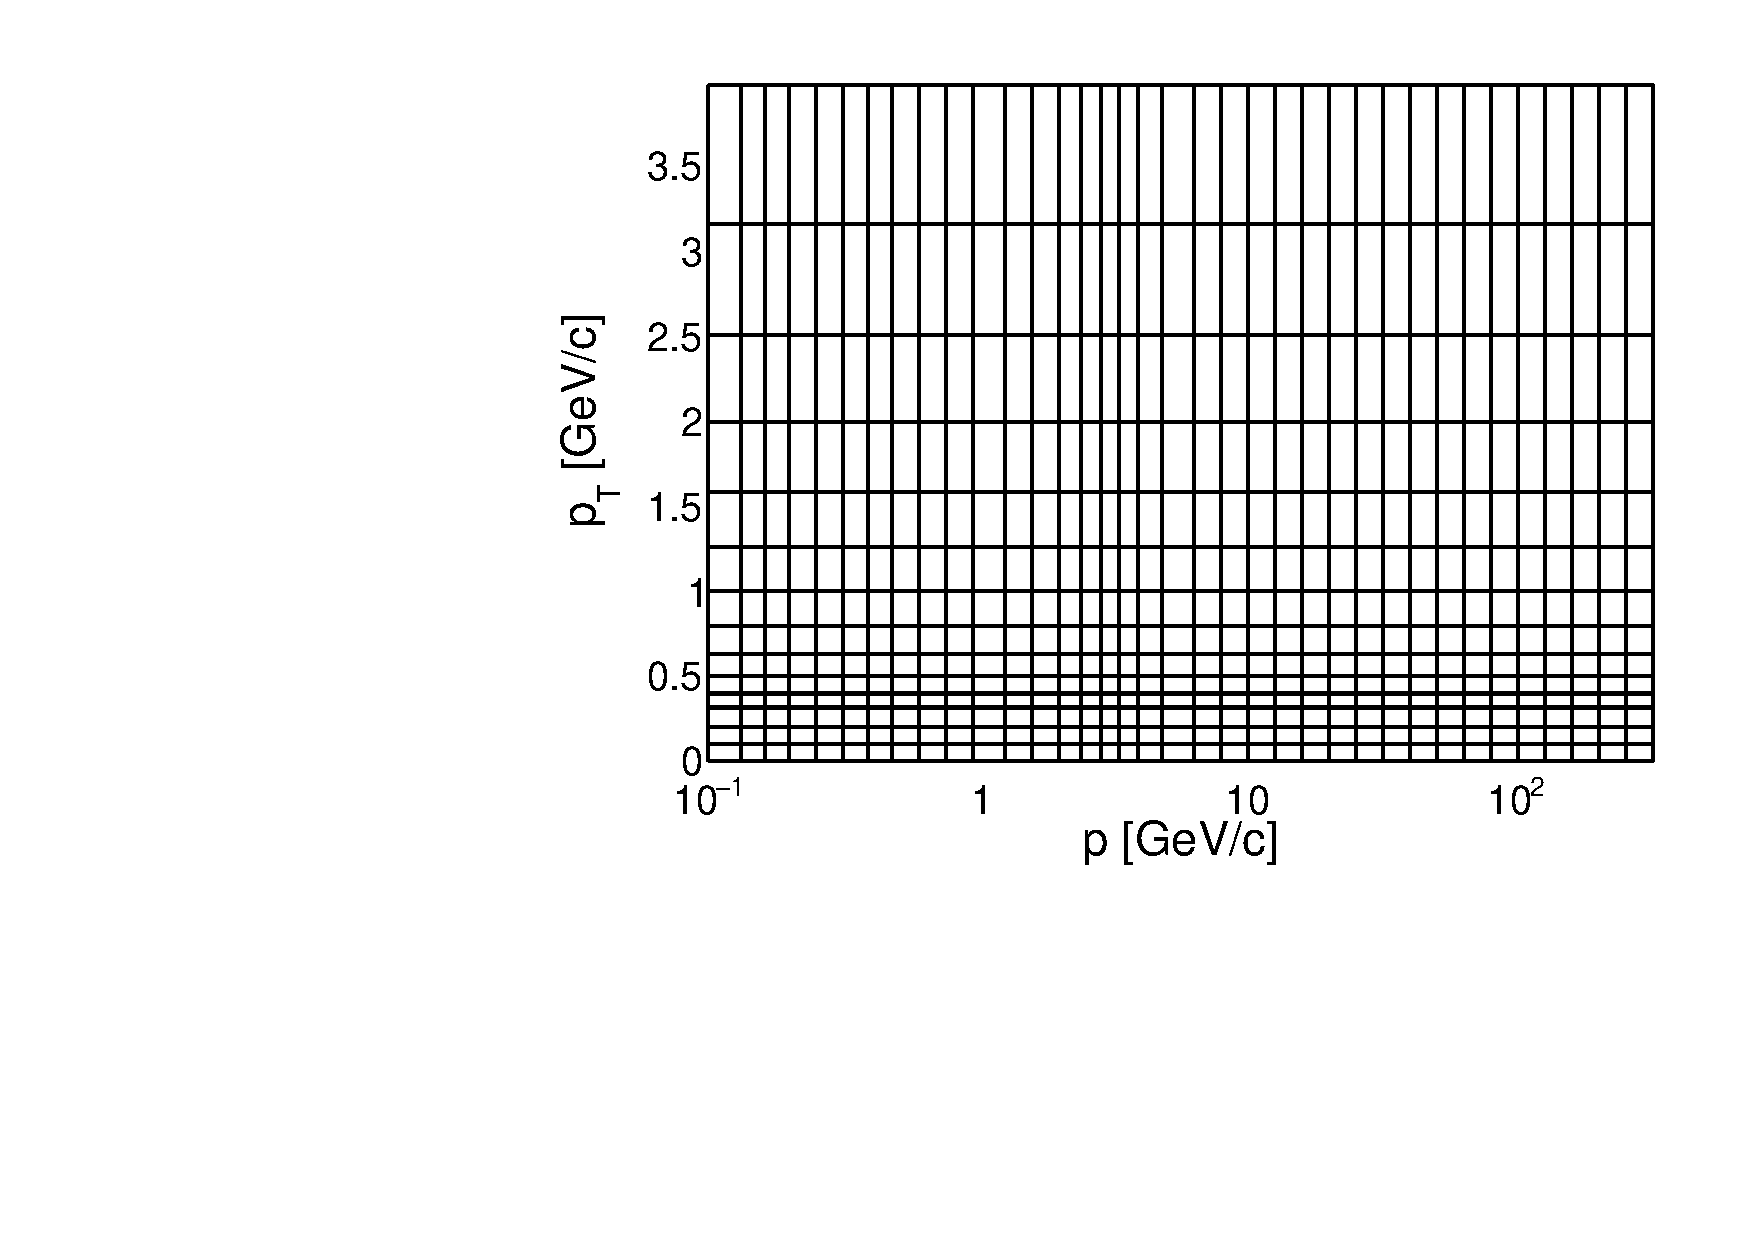
\includegraphics[clip, rviewport=0 0 1 1,width=0.5\textwidth]{DedxBinning}
  \caption{}
  \label{fig:hadron:binning:dedx}
\end{figure}

Since the \vzero analysis is done independently for the three target particles,
the phase space binning is not required to be unique. Because of statistics,
the number of bins defined for the \lamb and \antilamb is the same and
for \kzeros is larger than for the former ones.
In~\cref{fig:hadron:binning:vzero} we show the two
binning configuration for the \vzero analysis.

%%%%%%%%%%%%%% BINNING V0 %%%%%%%%%%%%%%%
\begin{figure}[!ht]
  \centering
  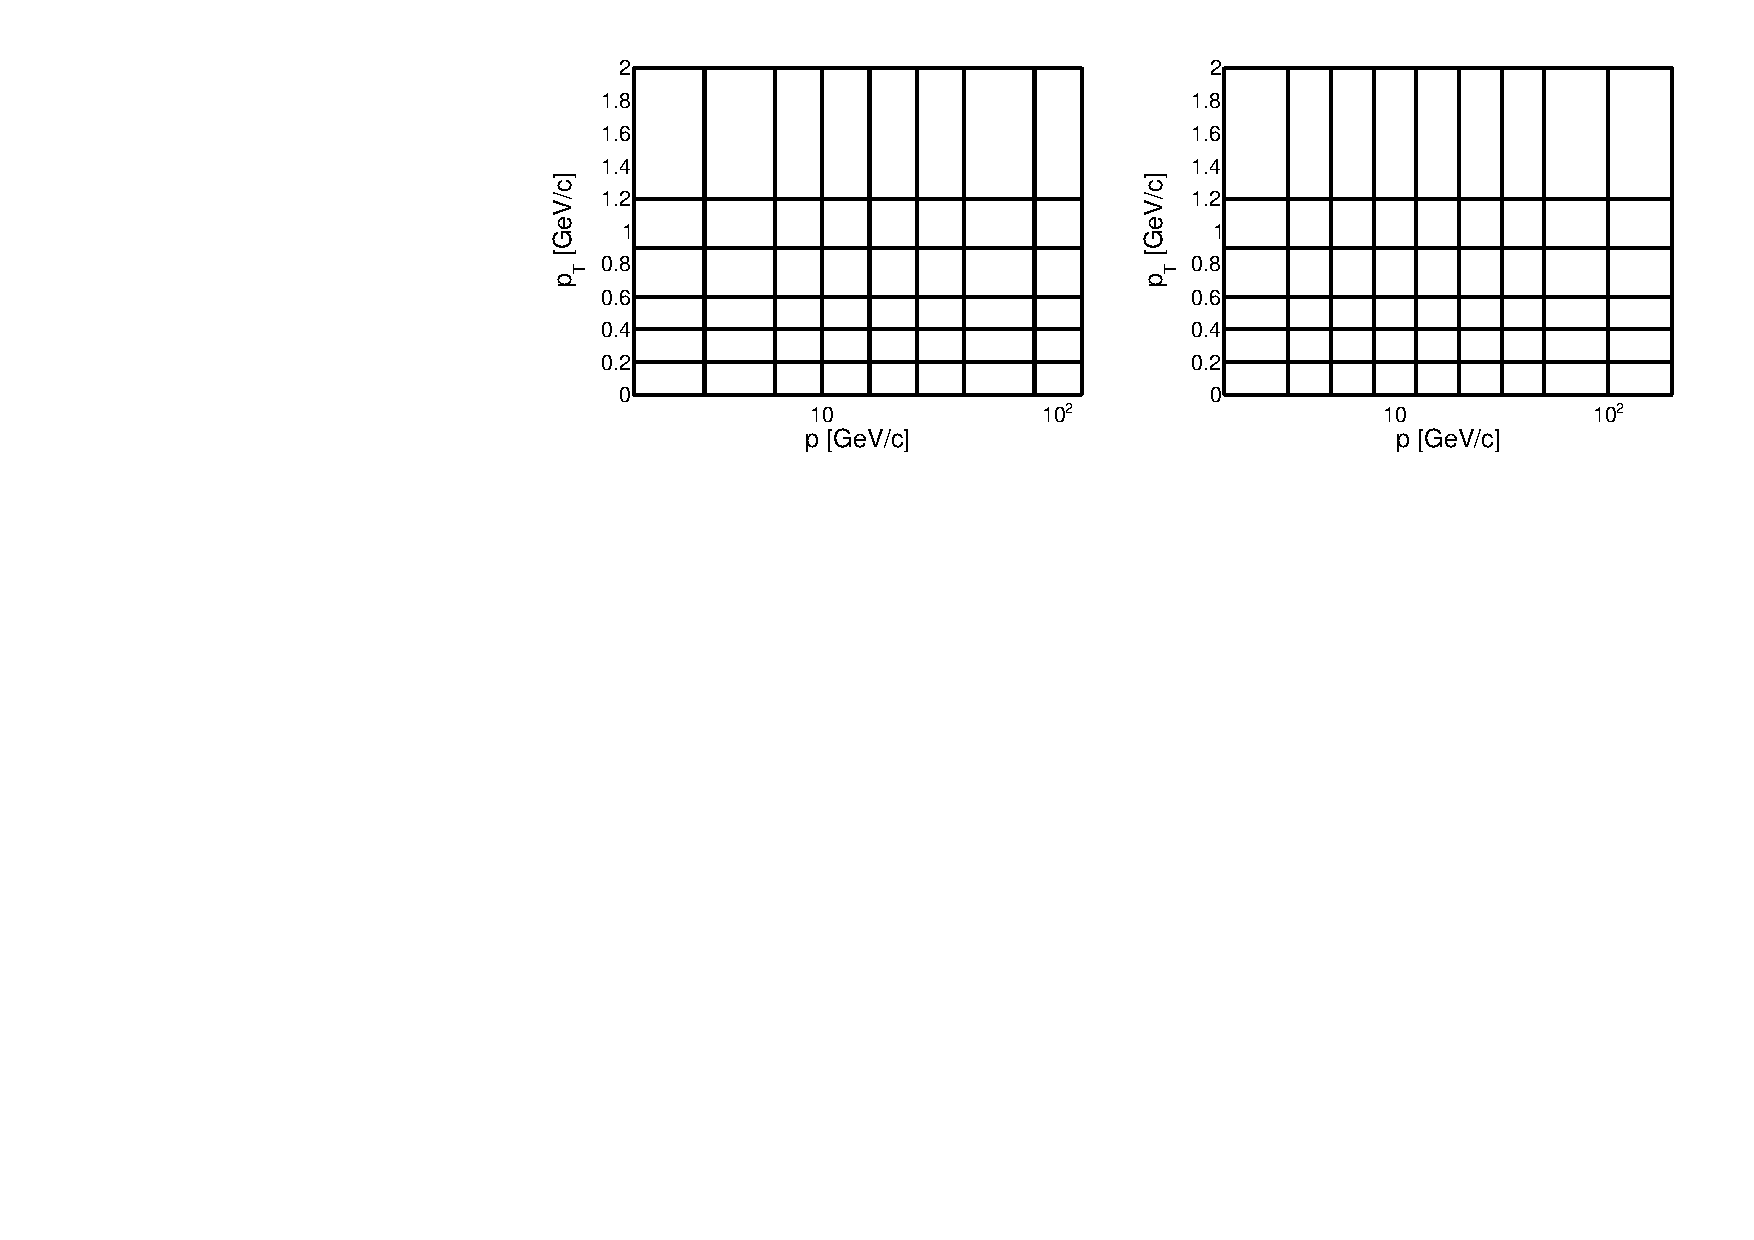
\includegraphics[clip, rviewport=0 0 1 1,width=0.8\textwidth]{V0Binning}
  \caption{}
  \label{fig:hadron:binning:vzero}
\end{figure}


%%%%%%%%%%%%%%%%%%%%%%%%%%%%%%%%%%%%%%%%
\section{Particle identification for the identified spectra}

\note{DONE}

In this section we present the particle identification
analysis for the identified spectra of \pions, \kaons and \protons.
This step is done in a track basis through the \dedx measurements,
being the aim here to determine the fraction of tracks which
correspond to each particle type on every phase space bin.
A brief overview of the \dedx measurements is first given
in~\cref{sec:hadron:dedx:meas}.

The \dedx measurements only allow the particle identification
to be done statistically by fitting
the \dedx distributions with a combination of particle
types. Because of the complicated dependence of the \dedx
distributions on the particle momentum,
features of the measured track (e.g. number of clusters) and
detector properties (e.g. resolution and calibration),
the \dedx fit turns to be very challenging. The first
requirement to perform this step is the development
of a appropriate \dedx model,
which is shown in~\cref{sec:hadron:dedx:model}.

Having in hands the \dedx model, the measured \dedx
distributions can be fitted to determine the particle
fractions. However, the usual large number of
model parameters, added to the
overlap of the \dedx distributions
of different particles in certain regions of momentum,
can make the this fit very hard to perform.
Our fit strategy to overcome these difficulties is shown
in~\cref{sec:hadron:dedx:fit}. A new tool
developed in this work to evaluate the fit performance
and estimated bias and statistical uncertainties of the fit
is presented in~\cref{sec:hadron:dedx:sde}. 
Finally, in~\cref{sec:hadron:dedx:results} we show the results
of the particle identification analysis.


%%%---------------------------------%%%%
\subsection{\dedx measurements}
\label{sec:hadron:dedx:meas}

\cite{Alt:2005zq}

\cite{BlumBook}

\warning{rewrite}

The \dedx associated to each track is defined as the energy lost by the charged
particle per unit of length.
In \NASixtyOne the \dedx is measured by the TPCs, which collect the number of
freed electrons from the ionization of the gas by the passage of the charged particles.
The determination of the \dedx from the signal recorded at the TPCs requires a complex and
detailed procedure, which has been very well established by the \NAFortyNine and \NASixtyOne
experiment along the last decades. Since the detailed description of this procedure
is out of the scope of this text, only the general idea and the most important aspects
will be presented in the next paragraphs. More complete and detailed approaches
can be found in Refs.\cite{LeeuwenThesis,GaborVeresThesis}.

Several processes can contribute to the energy loss of charged particle due to
its interaction with atoms of the gas in the TPCs, being the emission of
electrons by ionization the most relevant one. The electrons emitted are
drifted through the chamber and collected in the readout pads, which records
the signal as ADC charges. A set of consecutive charges defines a cluster.
The 3-dimensional position of the cluster is determined by the position
and time distributions in which the charges reaches the readout pad. This
position gives the crossing point of the particle track inside the TPCs.

The total charge measured in each cluster is related to the \dedx of each track.
However, numerous detector effects have to be corrected at the cluster level before
grouping the cluster in one unique \dedx value. The simplest correction accounts for
the geometrical differences due to the incident angle of the track in the pad and
the pad widths. More complicated corrections account for differences in the electronic
gain and gas pressure/temperature of the pads, differences in the sector gains and
losses of electrons during the drift in the chambers and in the readout pad.
A detailed description of the correction procedure can be found in Ref.~\cite{AntoniMThesis}.

The track \dedx is then determined by the combination of the corrected 
charges in all clusters. The well known Landau-like shape of the
energy loss probability distribution makes the simplest approach,
based on the average over all clusters, not suitable. Because of the
long tail of the probability distribution, the average and the variance
of the measured charges are not well behaved for typical number of clusters
($\sim$ 20-150). To overcome this issue and obtain a satisfactory \dedx resolution,
the method of the truncated mean is applied, in which only a subset of the clusters
is selected to compute the average. The selected clusters are defined by ordering
the values of the charge and the selecting the ones inside a given percentage interval.
For the \NASixtyOne experiment, it was found the optimal interval being the smallest 50\%
of the clusters~\cite{GaborVeresThesis}.


%%%---------------------------------%%%%
\subsection{\dedx model}
\label{sec:hadron:dedx:model}

\warning{rewrite}

To perform the particle identification by fitting the
measured \dedx distribution, a model that describe
the \dedx distributions of different particle types as a function
of their momentum \p is required. Once there is no universal choice
of this model, several different alternatives have been
used in previous analysis. Although the model chosen here 
is based on previous studies developed for
\NAFortyNine and \NASixtyOne experiment, it contain
particular features which were found to be the most suitable
for the present analysis.

First, the notation adopted in this text has to be presented
for clarification. The particle types are represented by
the index \ipart, and it can assume one of the five particle types
treated here, $\ipart=e, \pi, K, p, d$. The charges are represented by
the index \ich, being that $\ich = +$ or $\ich=-$. Also, the number of
cluster measured in a track is represented by \ncl and the \dedx
is replaced by \eps for simplicity.

Because the \dedx is obtained by averaging the measured charge
over a certain number of cluster, it is natural to assume that
the shape of the \eps distribution depends on the \ncl.
To be more precise, the \eps resolution should be 
larger for smaller \ncl and vice-versa. 
Additionally, it is obviously expected the mean of the distribution
to change with the momentum of the particle \p and the particle type.

Since the shape of the \eps distribution, for a given \ncl and \p,
can be well described by an asymmetric Gaussian function, the
probability density function of \eps for a particle type
\ipart and charge \ich is written as
\begin{equation}
  f_{\ipart,\ich}(\eps|\p,\ncl) = \frac{1}{\sqrt{2\pi}\sigma_{\ipart,\ich}} \;
  \exp\left[-\frac{1}{2}\left(\frac{\eps-\mu_{\ipart,\ich}}{\delta \; \sigma_{\ipart,\ich}}\right)^2\right],
  \label{eq:dedx:model:pdf}
\end{equation}
with
\begin{equation}
  \delta =
  \begin{cases}
    & 1-d, \ \ \ \eps \le \mu_{\ipart,\ich} \\
    & 1+d, \ \ \ \eps > \mu_{\ipart,\ich}, \\
  \end{cases}
  \label{eq:dedx:model:asymm}
\end{equation}
where the parameter $\mu$ is the mode of the distribution, $\sigma$ is the resolution
and $d$ is the asymmetry parameter. The \p and \ncl dependence is implicit
on the parameters $\mu$ and $\sigma$, as will be explained next.
The mode $\mu$ is related to the mean of the distribution, \meaneps, by
\begin{equation}
  \mu_{\ipart,\ich} = \meaneps_{\ipart,\ich} - \frac{\sigma_{\ipart,\ich}}{\sqrt{2\pi}}
  \left[\left(1+d\right)^2 - \left(1-d\right)^2 \right].
  \label{eq:dedx:model:mu}
\end{equation}

The \p evolution of \meaneps is expected to follow
a Bethe-Bloch-like function. In this model, a reference
\meaneps(\p) curve is defined by a data-based
parametrization using a generic function which is a
variation of the Bethe-Bloch function. The reference value
of \meaneps for a given \p is denoted as \meanepsbb.
To account for deviations from the reference \meaneps,
the present model includes a set of parameters called
\textit{calibration constants}, which are denoted by $X$.
These parameters act as logarithmic shifts of the \meaneps
around \meanepsbb and they can in principle be applied
to each particle and charge separately. To reduce the complexity
of the model, it is assumed here one global calibration constant
for each charge that follows the \meaneps of the $\pi$ distribution
and individual calibration constants for the other particles,
but being common for both charges. In the end, the \meaneps for a
given particle type \ipart and charge \ich is given by
\begin{equation}
  \meaneps_{\ipart,\ich} =
  \begin{cases}
    & \meaneps_{\ipart}^\text{BB} \; e^{X_{\ipart}^{\ich}} \ \ \ \ \ \ \ (i=\pi) \\
    & \meaneps_{\ipart}^\text{BB} \; e^{X_{\pi}^{\ich}} \; e^{X_{\ipart}^{\ich}} \ \ \ (i\neq\pi).
  \end{cases}
  \label{eq:dedx:model:cal}
\end{equation}
In total, 6 calibration constants are included in the model:
$X_{\pi}^{+}$, $X_{\pi}^{-}$, $X_{e}$, $X_{K}$, $X_{p}$ and $X_{d}$.

The dependence of the resolution $\sigma$ on \ncl is assumed to be of the form
$\sigma \sim 1/\sqrt{\ncl}$. Besides that, $\sigma$ is assumed to depend
on the \meaneps by a power law relation and a normalization parameter for
each charge is also included ($\sigma_0^{\ich}$). The final expression for the resolution is,
\begin{equation}
  \sigma_{\ipart,\ich} = \frac{\sigma_0^{\ich}}{\sqrt{\ncl}} \meaneps_{\ipart,\ich}^{\alpha},
  \label{eq:dedx:model:sigma}
\end{equation}
in which 3 more parameters are included: $\sigma_0^+$, $\sigma_0^-$ and $\alpha$. 

By combining
the~\cref{eq:dedx:model:asymm,eq:dedx:model:mu,eq:dedx:model:cal,eq:dedx:model:sigma}
with the~\cref{eq:dedx:model:pdf}, we obtain the probability density
function of \eps for each particle \ipart and charge \ich. Besides the 6 calibration constants,
the model includes 4 \textit{shape parameters}: $\sigma_0^+$, $\sigma_0^-$, $\alpha$ and $d$.
Altogether there are 10 parameters that can be set free to fit the model
to the measured \eps distributions.


%%%---------------------------------%%%%
\subsection{\dedx fit strategy}
\label{sec:hadron:dedx:fit}


%%%---------------------------------%%%%
\subsection{Simulated data ensembles, cuts and corrections}
\label{sec:hadron:dedx:sde}


%%%---------------------------------%%%%
\subsection{Particle identification results}
\label{sec:hadron:dedx:results}



%%%%%%%%%%%%%%%%%%%%%%%%%%%%%%%%%%%%%%%%
\section{\vzero analysis}


%%%---------------------------------%%%%
\subsection{Signal extraction}


\subsubsection{\vzero cuts}
\label{sec:hadron:signal:cuts}

%%%%%%%%%%%%%%%%%%%%%%%%%%%%%%%%%%%%%%%%
\section{Corrections}


%%%%%%%%%%%%%%%%%%%%%%%%%%%%%%%%%%%%%%%%
\section{Spectra}


%%%---------------------------------%%%%
\subsection{Statistical uncertainties}


%%%---------------------------------%%%%
\subsection{Systematic uncertainties}
\label{sec:hadron:spec:syst}



%%%%%%%%%%%%%%%%%%%%%%%%%%%%%%%%%%%%%%%%
\section{Results}

%%%%%%%%%%%%%%%%%%%%%%%%%%%%%%%%%%%%%%%%
\section{Summary and conclusions}

